\documentclass[class=minimal,border=0pt]{standalone}

\usepackage{tudfonts}

\usepackage{tikz}
\usetikzlibrary{calc}
\usetikzlibrary{matrix}
\usetikzlibrary{positioning}

\begin{document}

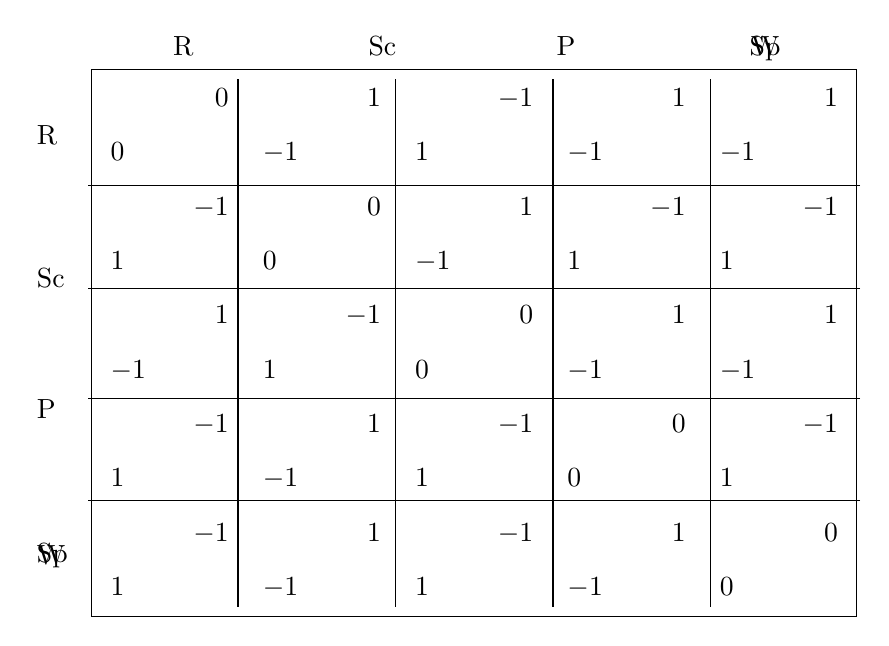
\begin{tikzpicture}

\matrix[matrix of math nodes,every odd row/.style={align=right},every even row/.style={align=left},every node/.style={text width=1.5cm},row sep=0.2cm,column sep=0.2cm] (m) {
$0$&$1$&$-1$&$1$&$1$\\
$0$&$-1$&$1$&$-1$&$-1$\\
$-1$&$0$&$1$&$-1$&$-1$\\
$1$&$0$&$-1$&$1$&$1$\\
$1$&$-1$&$0$&$1$&$1$\\
$-1$&$1$&$0$&$-1$&$-1$\\
$-1$&$1$&$-1$&$0$&$-1$\\
$1$&$-1$&$1$&$0$&$1$\\
$-1$&$1$&$-1$&$1$&$0$\\
$1$&$-1$&$1$&$-1$&$0$\\
};
\draw (m.north east) rectangle (m.south west);
\draw (m.north west)--(m.north west);
\draw (-3,3.35) -- (-3,-3.35);
\draw (1,3.35) -- (1,-3.35);
\draw (-1,3.35) -- (-1,-3.35);
\draw (3,3.35) -- (3,-3.35);

\draw (4.9,2) -- (-4.9,2);
\draw (4.9,0.7) -- (-4.9,0.7);
\draw (4.9,-0.7) -- (-4.9,-0.7);
\draw (4.9,-2) -- (-4.9,-2);


\coordinate (a) at ($(m.north west)!0.12!(m.north east)$);
\coordinate (b) at ($(m.north west)!0.38!(m.north east)$);
\coordinate (c) at ($(m.north west)!0.62!(m.north east)$);
\coordinate (d) at ($(m.north west)!0.88!(m.north east)$);
\coordinate (e) at ($(m.north west)!0.88!(m.north east)$);
\node[above=5pt of a,anchor=base] {R};
\node[above=5pt of b,anchor=base] {Sc};
\node[above=5pt of c,anchor=base] {P};
\node[above=5pt of d,anchor=base] {W};
\node[above=5pt of d,anchor=base] {Sp};

\coordinate (f) at ($(m.north west)!0.12!(m.south west)$);
\coordinate (g) at ($(m.north west)!0.38!(m.south west)$);
\coordinate (h) at ($(m.north west)!0.62!(m.south west)$);
\coordinate (i) at ($(m.north west)!0.888!(m.south west)$);
\coordinate (j) at ($(m.north west)!0.888!(m.south west)$);
\node[left=2pt of f,text width=.5cm]  {R};
\node[left=2pt of g,text width=.5cm]  {Sc};
\node[left=2pt of h,text width=.5cm]  {P};
\node[left=2pt of i,text width=.5cm]  {W};
\node[left=2pt of j,text width=.5cm]  {Sp};


\end{tikzpicture}

\end{document}
